%=======================================================================
\Tut\chapter{Kontextfreie Grammatiken}
\label{k:grammatiken}

%-----------------------------------------------------------------------
\Tut\section{Rekursive Definition syntaktischer Strukturen}

Wir hatten in \hyperref[k:dokumente]{Einheit~\ref{k:dokumente} über
  Dokumente} schon darauf hingewiesen, dass die Beschreibung formaler
Sprachen nur mit Hilfe einzelner Symbole und der Operation
Vereinigung, Konkatenation und Konkatenationsabschluss manchmal
möglich ist, aber manchmal anscheinend auch nicht.

Tatsächlich ist es manchmal unmöglich. Wie man zu einen harten Beweis
für diese Aussage kommen kann, werden wir in einer späteren Einheit
sehen.

Als typisches Beispiel eines Problemfalles sehen wir uns einen
Ausschnitt der Definition der Syntax von Java an (siehe die
Erläuterungen zu "`Blocks"' und "`Statements"' auf
\url{docs.oracle.com/javase/specs/jls/se7/html/jls-14.html},
18.10.13). Dort stehen im Zusammenhang mit der Festlegung, was in Java
eine Anweisung sei, unter anderem folgende fünf Teile:

\begin{table}[ht]
  \centering
  \begin{tabular}{l@{\hspace*{2em}}ll}
    \toprule
    1 & \multicolumn{2}{l}{Block:} \\
    & \hspace*{3em}& \literal{\{} BlockStatements\textsubscript{opt} \literal{\}} \\
    % 
    2 & \multicolumn{2}{l}{BlockStatements:} \\
    & & BlockStatement \\
    & & BlockStatements BlockStatement \\
    % 
    3 & \multicolumn{2}{l}{BlockStatement:} \\
    & & \dots \dots \\
    & & Statement \\
    4 & \multicolumn{2}{l}{Statement:} \\
    & & StatementWithoutTrailingSubstatement\\
    & & \dots \dots \\
    5 & \multicolumn{2}{l}{StatementWithoutTrailingSubstatement:} \\
    & & Block\\
    & & \dots \dots \\
    \bottomrule
  \end{tabular}
  \caption{Auszug aus der Spezifikation der Syntax von Java}
  \label{tab:java-grammar}
\end{table}

\noindent

Wir werden die Wörter aus obiger Spezifikation von normalem Text
unterscheiden, indem wir sie in spitzen Klammern und kursiv setzen,
wie \zB bei \meta{Block}, um das Lesen zu vereinfachen (und um schon
mal deutlich zu machen, dass es sich \zB bei \meta{Block} um etwas
handelt, was wir als \emph{ein} Ding ansehen wollen).

Man macht keinen Fehler, wenn man das zum Beispiel erst mal so liest:

%
\begin{enumerate}
\item Ein \meta{Block} hat die Struktur: Ein Zeichen \literal{\{} ,
  eventuell gefolgt von \meta{BlockStatements} (das tiefgestellte
  Suffix "`opt"' besagt, dass das optional ist), gefolgt von einem
  Zeichen \literal{\}}\ .
\item \meta{BlockStatements} sind von einer der Strukturen
  \begin{itemize}
  \item ein einzelnes \meta{BlockStatement} oder
  \item \meta{BlockStatements} gefolgt von einem \meta{BlockStatement}
  \end{itemize}
\item Ein \meta{BlockStatement} kann (unter anderem \dots) ein
  \meta{Statement} sein.
\item Ein \meta{Statement} kann ein
  \meta{Statement\-Without\-Trailing\-Sub\-state\-ment} sein (oder
  anderes, zum Beispiel etwas "`ganz einfaches"' \dots).
\item Ein \meta{StatementWithoutTrailingSubstatement} kann ein
  \meta{Block} sein (oder anderes \dots).
\end{enumerate}
%
Diese Formulierungen beinhalten Rekursion: Bei der Beschreibung der
Struktur von \meta{BlockStatements} wird direkt auf
\meta{Block\-State\-ments} Bezug genommen.

Außerdem wird bei der Definition von \meta{Block} (indirekt) auf
\meta{State\-ment} verwiesen und bei der Definition von
\meta{Statement} (indirekt) wieder auf \meta{Block}.

Wir werden uns der Antwort auf die Frage, wie man diese Rekursionen
eine vernünftige Bedeutung zuordnen kann, in mehreren Schritten
nähern.

Als erstes schälen wir den für uns gerade wesentlichen Aspekt noch
besser heraus. Schreiben wir einfach $X$ statt \meta{Block},
\meta{State\-ment} o.ä., und schreiben wir lieber runde Klammern
\literal{(} und \literal{)} statt der geschweiften, weil wir die die
ganze Zeit als Mengenklammern benutzen wollen. (Sie fragen sich, warum
nicht einen Ausschnitt aus der Grammatik für arithmetische Ausdrücke
genommen haben, in denen sowieso schon runde Klammern benutzt werden?
Die Antwort ist: Der Ausschnitt aus der Syntaxbeschreibung wäre viel
länger und unübersichtlicher geworden.)

Dann besagt die Definition unter anderem:
%
\begin{itemize}
\item[K1]\label{K1} Ein $X$ kann etwas "'ganz einfaches"' sein. Im
  aktuellen Zusammenhang abstrahieren wir mal ganz stark und schreiben
  für dieses Einfache einfach das leere Wort $\eps$.
\item[K2]\label{K2} Ein $X$ kann ein $Y$ sein oder auch ein $X$
  gefolgt von einem $Y$; also kann ein $X$ von der Form $YY$ sein.
  Jedes $Y$ seinerseits kann wieder ein $X$ sein. Also kann ein $X$
  auch von der Form $XX$ sein.
\item[K3]\label{K3} Wenn man ein $X$ hat, dann ist auch
  $\literal{(}X\literal{)}$ wieder ein $X$.
\item[K4]\label{K4} Schließlich tun wir so, als dürfe man in die
  Definition auch hineininterpretieren: Es ist nichts ein $X$, was man
  nicht auf Grund der obigen Festlegungen als solches identifizieren
  kann.
\end{itemize}
%
Und nun? Wir könnten jetzt zum Beispiel versuchen, mit $X$ eine
formale Sprache $L$ zu assoziieren, und folgende Gleichung
hinschreiben:
\begin{equation}
L = \{ \eps \} \cup LL \cup \{\literal{(}\} L \{\literal{)}\}
\label{eq:klammern}
\end{equation}
Dabei wäre die Hoffnung, dass die Inklusion $L\supseteq \dots$ die
ersten drei aufgezählten Punkte widerspiegelt, und die Inklusion
$L\subseteq \dots$ den letzten Punkt. Wir werden sehen, dass diese
Hoffnung zum Teil leider trügt.

Die entscheidenden Fragen sind nun natürlich:
%
\begin{enumerate}
\item Gibt es überhaupt eine formale Sprache, die
  Gleichung~\ref{eq:klammern} erfüllt? 

  Das hätten wir gerne, und wir werden sehen, dass es tatsächlich so
  ist, indem wir eine Lösung der Gleichung konstruieren werden.
\item Und falls ja: Ist die formale Sprache, die
  Gleichung~\ref{eq:klammern} erfüllt, nur durch die Gleichung
  eindeutig festgelegt? 

  Das hätten wir auch gerne, wir werden aber sehen, dass das
  \emph{nicht} so ist.  Das bedeutet für uns die zusätzliche Arbeit,
  dass wir "`irgendwie"' eine der Lösungen als die uns interessierende
  herausfinden und charakterisieren müssen. Das werden wir im nächsten
  Unterabschnitt machen.
\end{enumerate}
% 
Zum Abschluss dieses Unterabschnittes wollen wir eine Lösung von
Gleichung~\ref{eq:klammern} konstruieren.  Wie könnte man das tun?
Wir "`tasten uns an eine Lösung heran"'.

Das machen wir, indem wir
\begin{itemize}
\item erstens eine ganze Folge $L_0$, $L_1$, \dots\ formaler Sprachen
  $L_i$ für $i\in\N_0$ definieren, der Art, dass jedes $L_i$
  offensichtlich jedenfalls einige der gewünschten Wörter über dem
  Alphabet $\{\literal{(}, \literal{)}\}$ enthält, und
\item zweitens dann zeigen, dass die Vereinigung aller dieser $L_i$
  eine Lösung von Gleichung~\ref{eq:klammern} ist.
\end{itemize}
%
Also:
%
\begin{itemize}
\item Der Anfang ist ganz leicht: $L_0 = \{\eps\}$.
\item und weiter machen kann man so: für $i\in\N_0$ sei \\
  $L_{i+1}= L_iL_i \cup \{\literal{(}\} L_i \{\literal{)}\}$.
\end{itemize}
%
Wir behaupten, dass $L=\bigcup_{i=0}^{oo} L_i$
Gleichung~\ref{eq:klammern} erfüllt.

Zum Beweis der Gleichheit überzeugen wir uns davon, dass beide
Inklusionen erfüllt sind. 

Zunächst halten wir fest: $\eps\in L_0$. Außerdem ist für alle $i\in
\N_0$ auch $L_iL_i\subseteq L_{i+1}$, wenn also $\eps\in L_i$, dann
auch $\eps=\eps\eps\in L_iL_i$, also $\eps\in L_{i+1}$. Also gilt für
alle $i\in \N_0$: $\eps\in L_i$.  Und folglich gilt für alle
$i\in\N_0$: $L_i=L_i\{\eps\}\subseteq L_i L_i$, also ist für alle
$i\in\N_0$: $L_i\subseteq L_{i+1}$.

\begin{description}
\item[$L\subseteq \{ \eps \} \cup LL \cup \{\literal{(}\} L
  \{\literal{)}\}$:] Da $\eps\in L_0\subseteq L$ ist, ist
  $L=L\{\eps\}\subseteq LL$.
\item[$L\supseteq \{ \eps \} \cup LL \cup \{\literal{(}\} L
  \{\literal{)}\}$:] sei $w\in \{ \eps \} \cup LL \cup
  \{\literal{(}\} L \{\literal{)}\}$. 
  \begin{description}
  \item[1. Fall: $w=\eps$:] $w=\eps\in L_0\subseteq L$.
  \item[2. Fall: $w\in LL$:] Dann ist $w=w_1w_2$ mit $w_1\in L$ und
    $w_2\in L$. Es gibt also Indizes $i_1$ und $i_2$ mit $w_1\in
    L_{i_1}$ und $w_2\in L_{i_2}$. Für $i=\max(i_1,i_2)$ ist also
    $w_1\in L_i$ und $w_2\in L_i$, also $w=w_1w_2\in L_iL_i\subseteq
    L_{i+1}\subseteq L$.
  \item[3. Fall: $w\in \{\literal{(}\} L \{\literal{)}\}$:] Für ein
    $i\in \N_0$ ist dann $w\in \{\literal{(}\} L_i
    \{\literal{)}\}\subseteq L_{i+1}\subseteq L$.
  \end{description}
\end{description}
%
Damit haben wir gezeigt, dass Gleichung~\ref{eq:klammern} (mindestens)
eine Lösung hat.

Um zu sehen, dass die konstruierte Lösung keineswegs die einzige ist,
muss man sich nur klar machen, dass $\{\literal{(}, \literal{)}\}^*$
auch eine Lösung der Gleichung ist, aber eine andere.
\begin{itemize}
\item Dass es sich um eine Lösung handelt, sieht man so:
  "`$\subseteq$"' zeigt man wie oben; "`$\supseteq$"' ist trivial, da
  $\{\literal{(}, \literal{)}\}^*$ eben \emph{alle} Wörter sind.
\item Dass es eine andere Lösung ist, sieht man daran, dass \zB das
  Wort $\literal{(((}$ zwar in $\{\literal{(}, \literal{)}\}^*$ liegt,
  aber \emph{nicht} in der oben konstruierten Lösung. Die enthält
  nämlich jedenfalls nur Wörter, in denen gleich viele $\literal{(}$
  und $\literal{)}$ vorkommen. (Diese Behauptung gilt nämlich für alle
  $L_i$, wie man durch vollständige Induktion zeigen kann.)
\end{itemize}
%
Kommen wir zurück zu unserer zuerst konstruierten Lösung
$L=\bigcup_{i=0}^{\infty} L_i$.  Zählen wir für die ersten vier $L_i$
explizit auf, welche Wörter jeweils neu hinzukommen:
%
\begin{align*}
  L_0 &= \{ \eps \} \\
  L_1 \smallsetminus L_0 &=   \{ \;\literal{()} \;\} \\
  L_2 \smallsetminus L_1 &=   \{\; \literal{()()}\;,\; \literal{(())}\; \} \\
  L_3 \smallsetminus L_2 &= \{ 
  \begin{aligned}[t]
    &\;\literal{()()()}\; , 
    \;\literal{(())()}\; ,
    \;\literal{()(())}\; , \\
    &\;\literal{()()()()}\; ,
    \;\literal{()()(())}\; , 
    \;\literal{(())()()}\; , 
    \;\literal{(())(())}\; , \\
    &\; \literal{(()())}\; ,
    \; \literal{((()))}\; \left.\right\} \\
  \end{aligned} \\
\end{align*}
%
Dabei gilt zum Beispiel:
\begin{itemize}
\item Die Erklärung für $\literal{(())()()}\in L_3$ ist, dass
  $\literal{(())}\in L_2$ und $\literal{()()}\in L_2$ und Regel K2.
  \begin{itemize}
  \item Die Erklärung für $\literal{(())}\in L_2$ ist, dass 
    $\literal{()}\in L_1$ und Regel K3.
    \begin{itemize}
    \item Die Erklärung für $\literal{()}\in L_1$ ist, dass
      $\eps\in L_0$ und Regel K3.
    \end{itemize}
  \item Die Erklärung für $\literal{()()}\in L_2$ ist, dass
    $\literal{()}\in L_1$ und $\literal{()}\in L_1$ ist und Regel K2
    \begin{itemize}
    \item Die Erklärung für $\literal{()}\in L_1$ ist, dass
      $\eps\in L_0$ und Regel K3.
    \item Die Erklärung für $\literal{()}\in L_1$ ist, dass
      $\eps\in L_0$ und Regel K3.
    \end{itemize}
  \end{itemize}
\end{itemize}
%
Das kann man auch in graphischer Form darstellen: siehe
Abbildung~\ref{fig:baum-begruendung}. Ersetzt man dann noch überall
die $w\in L_i$ durch "`$X$"', ergibt sich
Abbildung~\ref{fig:abl-baum-informell}.

\begin{figure}[ht]
  \centering
  
  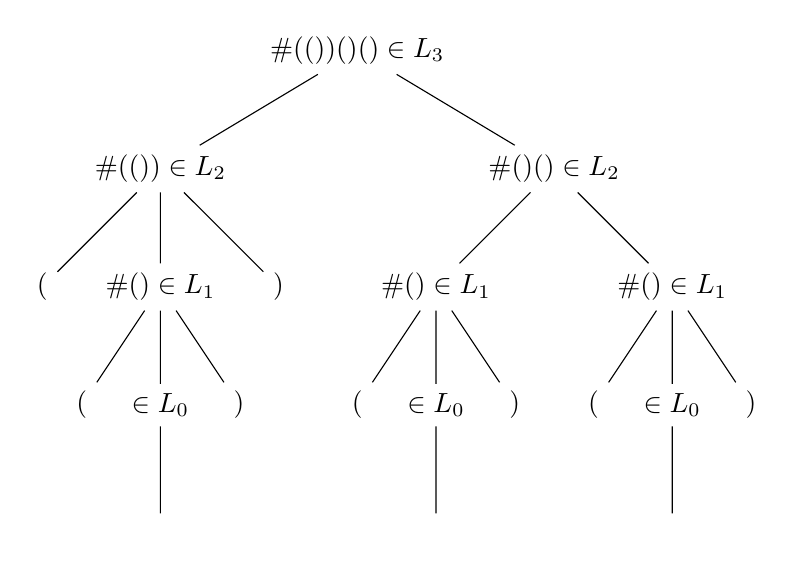
\begin{tikzpicture}
    [level 1/.style={sibling distance=50mm},
     level 2/.style={sibling distance=30mm},
     level 3/.style={sibling distance=10mm}]
    \node {$\#{(())()()}\in L_3$}
      child { node {$\#{(())}\in L_2$}
        [level 2/.style={sibling distance=15mm}]
        child {node {$\literal{(}$} }
        child {node {$\#{()}\in L_1$} 
          child {node {$\literal{(}$} }
          child {node {$\eps\in L_0$}
            child {node {$\eps$} }
          }
          child {node {$\literal{)}$} }
        }
        child {node {$\literal{)}$} }
      } 
      child { node {$\#{()()}\in L_2$} 
        child { node {$\#{()}\in L_1$} 
          child {node {$\literal{(}$} }
          child {node {$\eps\in L_0$}
            child {node {$\eps$} }
          }
          child {node {$\literal{)}$} }
        }
        child { node {$\#{()}\in L_1$} 
          child {node {$\literal{(}$} }
          child {node {$\eps\in L_0$}
            child {node {$\eps$} }
          }
          child {node {$\literal{)}$} }
        }
      } ;
  \end{tikzpicture}
  \caption{Eine "`Begründung"', warum $\literal{(())()()}\in L_3$ ist.} %
  \label{fig:baum-begruendung}
\end{figure}

\begin{figure}[ht]
  \centering
  
  \begin{tikzpicture}
    [level 1/.style={sibling distance=50mm},
     level 2/.style={sibling distance=30mm},
     level 3/.style={sibling distance=10mm}]
    \node {$X$}
      child { node {$X$}
        [level 2/.style={sibling distance=15mm}]
        child {node {$\literal{(}$} }
        child {node {$X$} 
          child {node {$\literal{(}$} }
          child {node {$X$}
            child {node {$\eps$} }
          }
          child {node {$\literal{)}$} }
        }
        child {node {$\literal{)}$} }
      } 
      child { node {$X$} 
        child { node {$X$} 
          child {node {$\literal{(}$} }
          child {node {$X$}
            child {node {$\eps$} }
          }
          child {node {$\literal{)}$} }
        }
        child { node {$X$} 
          child {node {$\literal{(}$} }
          child {node {$X$}
            child {node {$\eps$} }
          }
          child {node {$\literal{)}$} }
        }
      } ;
  \end{tikzpicture}
  \caption{Eine abstraktere Darstellung der "`Begründung"', warum
    $\literal{(())()()}\in L_3$ ist.} %
  \label{fig:abl-baum-informell}
\end{figure}

Eine solche Darstellung nennt man in der Informatik einen Baum
(kurioserweise wird die "`Wurzel"' üblicherweise oben dargestellt und
die "`Blätter"' unten). Auf Bäume und andere Graphen als
Untersuchungsgegenstand werden wir in einer späteren Einheit zu
sprechen kommen. Vorläufig genügt es uns, dass wir solche Bilder malen
können.

Zu kontextfreien Grammatiken ist es nun nur noch ein kleiner Schritt:
Statt wie eben im Baum Verzweigungen von unten nach oben als
Rechtfertigungen zu interpretieren, geht man umgekehrt vor und
interpretiert Verzweigungen als Stellen, an denen man
"`Verfeinerungen"' vornimmt, indem man rein syntaktisch zum Beispiel
ein $X$ \emph{ersetzt} durch $\literal{(} X \literal{)}$ oder $XX$.

%-----------------------------------------------------------------------
\Tut\section{Kontextfreie Grammatiken}

Eine \mdefine{kontextfreie Grammatik}\index{kontextfreie
  Grammatik}\index{Grammatik!kontextfreie} $G=(N,T,S,P)$ ist durch
vier Bestandteile gekennzeichnet, die folgende Bedeutung haben:
%
\begin{itemize}
\item $N$ ist ein Alphabet, dessen Elemente
  \mdefine{Nichtterminalsymbole}\index{Nichtterminalsymbol} heißen.
\item $T$ ist ein Alphabet, dessen Elemente
  \mdefine{Terminalsymbole}\index{Terminalsymbol} heißen. Kein Zeichen
  darf in beiden Alphabeten vorkommen; es muss stets $N\cap
  T=\emptyset$ sein.
\item $S\in N$ ist das sogenannte
  \mdefine{Startsymbol}\index{Startsymbol} (also ein
  Nichtterminalsymbol).
\item $P\subseteq N \x V^*$ ist eine \emph{endliche} Menge sogenannter
  \mdefine{Produktionen}\index{Produktion}. Dabei ist $V=N\cup T$ die
  Menge aller Symbole überhaupt.
\end{itemize}
%
Gilt für ein Nichtterminalsymbol $X$ und ein Wort $w$, dass $(X,w)\in
P$ ist, dann schreibt man diese Produktion üblicherweise in der Form
\mdefine{$X->w$} auf. Eine solche Produktion besagt, dass man ein
Vorkommen des Zeichens $X$ durch das Wort $w$ ersetzen darf, und zwar
"`egal wo es steht"', \dh ohne auf den Kontext zu achten.  

Das ist dann das, was man einen
\mdefine{Ableitungsschritt}\index{Ableitungsschritt} gemäß einer
Grammatik nennt. Formal definiert man das so: Aus einem Wort $u\in
V^*$ ist in einem Schritt ein Wort $v\in V^*$ ableitbar, in Zeichen
\mdefine{$u=> v$}, wenn es Wörter $w_1,w_2\in V^*$ und eine Produktion
$X->w$ in $P$ gibt, so dass $u=w_1Xw_2$ und $v=w_1ww_2$.
%
\begin{tutorium}
  \noindent
  \textbf{Beispielgrammatiken}
  \begin{itemize}
  \item Bitte auf den Unterschied zwischen dem einfachen Pfeil $->$
    bei Produktionen und dem Doppelpfeil $=>$ bei Ableitungsschritten
    achten (kann doch nicht so schwer sein, die Vorlesung ist doch so
    leicht ;=) )

    Beachte: Wenn $w_1->w_2$ gilt, dann auch $w_1=>w_2$, aber nicht
    unbedingt umgkehrt, wie man an der Grammatik $(\{X,Y\}, \{\#a\}, X
    \{X->Y, Y->\#a\})$ sieht:
    \begin{itemize}
    \item Es gilt z.B.\ $XY=> X\#a$, aber es gibt keine Produktion
      $XY-> X\#a$
    \end{itemize}
  \item arbeiten Sie ein bisschen mit $G=(\{X\}, \{\#a, \#b\}, X, \{X
    -> \eps \;|\; \#aX \;|\; \#bX \})$
    \begin{itemize}
    \item Was kann man alles ableiten? $\eps$, \#a, \#b, \#{aa}, \dots
    \item aha: alle Wörter überhaupt: $L(G)=\{\#a, \#b\}^*$
    \end{itemize}
  \item Gibt es auch eine Grammatik $G$ mit  $L(G)=\{\}$?
    \begin{itemize}
    \item suchen lassen \dots
    \item \zB $(\{X\}, \{\#a, \#b\}, X, \{X -> X\})$.
    \item wir haben sogar leere Produktionenmenge zugelassen: $(\{X\},
      \{\#a, \#b\}, X, \{\})$ tuts auch.
    \item allerdings: leere Alphabete haben wir verboten, also $(\{X\},
      \{ \}, X, P)$ geht \emph{nicht}.
    \end{itemize}
  \item Man arbeite mit $G=(\{X\}, \{ \#(, \#)\}, X, \{X -> XX
    \;|\; \#( X \#) \;|\; \eps \}$
    \begin{itemize}
    \item man mache Beispielableitungen
      \begin{itemize}
      \item erste einfache wie $X => \#(X\#) => \#(\#(X\#)\#) =>
        \#(\#(\#(X\#)\#)\#) => \#(\#(\#(\#(X\#)\#)\#)\#) =>
        \#(\#(\#(\#(\#)\#)\#)\#) $ oder
      \item $X => XX => XXX => XXXX => XXXXX$ und dann irgendwie weiter
      \end{itemize}
    \item Welche Wörter $w$ sind ableitbar?
      \begin{itemize}
      \item anschaulich: ableitbar sind genau die "`\emph{wohlgeformten
          Klammerausdrücke}"'
      \item jedenfalls gleich viele \#( und \#): $N_{\#(}(w) = N_{\#)}(w)$
      \item Das ist aber nur notwendig aber nicht hinreichend für
        Ableitbarkeit, denn \#{)(} ist \zB nicht ableitbar.
      \item Man diskutiere die Adjektive "`\emph{notwendig}"' und
        "`\emph{hinreichend}"'.
      \item zusätzliche Eigenschaften? erst mal raten/ nachdenken/
        rumprobieren lassen
      \item aha: für jedes Präfix (es heißt \emph{das} Präfix) $v$ eines
        $w\in L(G)$
        gilt: $N_{\#(}(v) \geq N_{\#)}(v)$\\
        Das kann man sich gerade noch klar machen; aber der Beweis, dass
        man damit eine notwendige und hinreichende Bedingung für
        Ableitbarkeit hat, also eine Charakterisierung der
        Klammerausdrücke, ist wohl zu schwierig; ich sehe jedenfalls auf
        Anhieb keine vernünftige Erklärung.
      \end{itemize}
    \end{itemize}
  \item Man arbeite mit $G=(\{X\}, \{ \#(, \#)\}, X, \{X -> \#(X\#)X \;|\;  \eps\})$.
    \begin{itemize}
    \item siehe da: auch damit sind genau die wohlgeformten Klammerausdrücke ableitbar
    \item Man mache sich klar, warum \dots
    \end{itemize}
  \item Und dann auch Grammatiken konstruieren \emph{lassen}, \zB für
    die folgenden formalen Sprachen über dem Alphabet $T=\{\#a,\#b\}$.
    \begin{itemize}
    \item die Menge aller Wörter über $T$, in denen irgendwo das
      Teilwort \#{baa} vorkommt, \\
      \zB so: $(\{X,Y\},T,X,P)$ mit $P=\{X->Y\#{baa}Y, Y ->\#aY|
      \#bY|\eps\}$
    \item die Menge aller Wörter $w\in T^*$ mit der Eigenschaft, dass
      für alle Präfixe $v$ von $w$ gilt: $|N_{\#a}(v) -N_{\#b}(v)| \leq
      1$. 
      \begin{itemize}
      \item Man überlege sich erst mal, welche Struktur Wörter der Länge
        $2$, $4$, \dots haben: wenn ich das richtig sehe: $\{\#{ab},
        \#{ba}\}^*$
      \item Also leistet die Grammatik $(\{X,Y\},T,X,P)$ mit
        $P=\{X->\#{ab}X|\#{ba}X|\#a|\#b|\eps\}$ das Gewünschte.
      \end{itemize}
    \end{itemize}
  \item \textbf{Achtung}: bitte nicht aus Versehen mit Grammatiken \bzw
    formalen Sprachen vom Aufgabenblatt~5 rumspielen
  \end{itemize}
\end{tutorium}

Betrachten wir als Beispiel die Grammatik $G=(\{X\},\{\literal{a},
\literal{b}\}, X, P)$ mit der Produktionenmenge $P=\{X-> \eps,
X->\literal{a} X\literal{b} \}$. Dann gilt zum Beispiel
$\#{aba}X\#{ba}XXXX => \#{aba}X\#{baa}X\#bXXX$, wie man an der
folgenden Aufteilung sieht:
\[
\underbrace{\literal{aba}X\literal{ba}}_{w_1}X\underbrace{XXX}_{w_2} 
=> \underbrace{\literal{aba}X\literal{ba}}_{w_1}\literal{a}X\literal{b}\underbrace{XXX}_{w_2} 
\]
Ebenso gilt $\#{aba}X\#{ba}XXXX => \#{abaa}X\#{bba}XXXX$:
\[
\underbrace{\literal{aba}}_{w_1}X\underbrace{\literal{ba}XXXX}_{w_2} 
=> \underbrace{\literal{aba}}_{w_1}\literal{a}X\literal{b}\underbrace{\literal{ba}XXXX}_{w_2} 
\]
Man kann also unter Umständen aus dem gleichen Wort verschiedene
Wörter in einem Schritt ableiten.

Die Definition von $=>$ legt eine Relation zwischen Wörtern über dem
Alphabet $V=N\cup T$ fest. Man könnte also auch schreiben: $R_{=>}
\subseteq V^*\x V^*$ oder gar $=> \subseteq V^*\x V^*$.  In diesem
Fall, wie \zB auch bei der $\leq$-Relation, ist es aber so, dass man
die sogenannte \mdefine{Infixschreibweise}\index{Infixschreibweise}
bevorzugt: Man schreibt $5 \leq 7$ und nicht $(5,7)\in R_{\leq}$
o.\;ä.
%
\begin{tutorium}
  \noindent
  \textbf{Infixschreibweise} von Relationen
  \begin{itemize}
  \item das kennt jeder von $x \leq y$ etc.
  \item sicherstellen, dass das klar ist: $x R y$ ist nichts anderes als $(x,y)\in R$
  \end{itemize}
\end{tutorium}
Im allgemeinen ist $=>$ weder links- noch rechtstotal und weder links-
noch rechtseindeutig.

Da die linke Seite einer Produktion immer ein Nichtterminalsymbol ist,
wird bei einem Ableitungsschritt nie ein Terminalsymbol ersetzt. Wo
sie stehen, ist "`die Ableitung zu Ende"' (daher der Name
\emph{Terminal}symbol). Eine \mdefine{Ableitung}\index{Ableitung}
(oder auch \define{Ableitungsfolge}\index{Ableitungsfolge}) ist eine
Folge von Ableitungsschritten, deren Anzahl irrelevant ist. Die
folgenden Definitionen kommen Ihnen vermutlich schon vertrauter vor
als vor einigen Wochen. Für alle $u,v\in V^*$ und für jedes
$i\in \N_0$ gelte
%
\begin{align*}
  u =>^0 v &\text{ genau dann, wenn } u=v \\
  u =>^{i+1} v &\text{ genau dann, wenn für ein}  w\in V^*: u => w =>^i v\\
  u =>^* v &\text{ genau dann, wenn für ein } i\in\N_0: u =>^i v \\
\end{align*}
%
Bei unserer Beispielgrammatik gilt zum Beispiel
\[
X => \literal{a}X\literal{b} 
=> \literal{aa}X\literal{bb}
=> \literal{aaa}X\literal{bbb}
=> \literal{aaa}\literal{bbb}
\]
%
Also hat man \zB die Beziehungen $X=>*\literal{aa}X\literal{bb}$,
$\literal{a}X\literal{b}=>* \literal{aaa}X\literal{bbb}$, $X =>*
\literal{aaabbb}$ und viele andere.  Weiter geht es in obiger
Ableitung nicht, weil überhaupt keine Nichtterminalsymbole mehr
vorhanden sind.
%
\begin{tutorium}
  \noindent
  \textbf{Unterschied $=>$ versus $=>*$}
  \begin{itemize}
  \item bitte sicherstellen, dass der Unterschied zwischen $=>$, also
    "`\emph{genau ein Schritt}"', und $=>*$, also "`\emph{eine
      beliebige Anzahl Schritte}"' klar ist.
  \end{itemize}
\end{tutorium}

Sozusagen das Hauptinteresse bei einer Grammatik besteht in der Frage,
welche Wörter aus Terminalsymbolen aus dem Startsymbol abgeleitet
werden können. Ist $G=(N,T,S,P)$, so ist die \mdefine{von einer
  Grammatik erzeugte formale Sprache}\index{erzeugte formale
  Sprache}\index{formale Sprache!erzeugte}
\[
L(G) = \{ w \in T^* \mid S =>* w \} \;.
\]
Eine formale Sprache, die man mit einer kontextfreien Grammatik
erzeugen kann, heißt auch \mdefine{kontextfreie Sprache}%
\index{kontextfreie Sprache}\index{formale Sprache!kontextfrei}.

Was ist bei unserer Beispielgrammatik $G=(\{X\},\{\literal{a},
\literal{b}\}, X, \{X-> \eps, X->\literal{a} X\literal{b} \}$? Eben
haben wir gesehen: $\literal{aaabbb}\in L(G)$. Die Ableitung ist so
strukturiert, dass man als Verallgemeinerung leicht sieht, dass für
alle $i\in\N_0$ gilt: $\literal{a}^i\literal{b}^i\in L(G)$. Der Beweis
(Sie wissen schon wie \dots) wird leichter, wenn man mit der
allgemeineren Behauptung beginnt:
\[
\forall i\in\N_0: ( X =>* \literal{a}^i\literal{b}^i 
\land X =>* \literal{a}^i X\literal{b}^i )
\]
Daraus folgt, dass $\{\literal{a}^i \literal{b}^i\mid
i\in\N_0\}\subseteq L(G)$ ist.  Umgekehrt kann man zeigen, dass gilt:
\[
\forall i\in\N_0: \text{ wenn } X =>^{i+1} w \text{, dann } w= \literal{a}^i
\literal{b}^i \lor w= \literal{a}^{i+1} X\literal{b}^{i+1}
\]
Daraus folgt $ L(G)\subseteq\{\literal{a}^i \literal{b}^i\mid
i\in\N_0\}$. Insgesamt ergibt sich also:
\[
L(G) = \{ \literal{a}^i\literal{b}^i \mid i\in\N_0 \} \;.
\]
%
Um eine etwas kompaktere Notation zu haben, fasst man manchmal mehrere
Produktionen mit gleicher linker Seite zusammen, indem man das
Nichtterminalsymbol und den Pfeil nur einmal hinschreibt, und die
rechten Seiten durch senkrechte Striche getrennt auf"|führt. Für
unsere Beispielgrammatik sieht die Produktionenmenge dann so aus:
\[
P = \{\;  X -> \literal{a} X \literal{b} \;|\; \eps \;\}
\]
%
Und  damit können  wir nun  auch die  richtige Interpretation  für die
Fragmente aus Tabelle~\ref{tab:java-grammar}  angeben: Es handelt sich
um Produktionen einer kontextfreien Grammatik.
%
\begin{itemize}
\item Jedes der Wörter "`Block"' ist \emph{ein} Nichtterminalsymbol.
  Deswegen haben wir Schreibweisen wie \meta{Block} vorgezogen, um
  deutlicher zu machen, dass wir so etwas als \emph{ein} nicht weiter
  zerlegbares Objekt betrachten wollen.
\item Der Doppelpunkt entspricht unserem Pfeil $->$ und trennt linke
  Seite einer Produktion von rechten Seiten.
\item Jede eingerückte Zeile ist eine rechte Seite einer Produktion.
\item Aufeinander folgende Zeilen muss man sich durch senkrechte
  Striche $|$ getrennt denken.
\end{itemize}
%
Der zweite Teil \\[0pt]

\begin{tabular}{l@{\hspace*{2em}}ll}
  \toprule
%  1 & \multicolumn{2}{l}{Block:} \\
%  & \hspace*{3em}& \literal{\{} BlockStatements\textsubscript{opt} \literal{\}} \\
  % 
  2 & \multicolumn{2}{l}{BlockStatements:} \\
  & \hspace*{3em} & BlockStatement \\
  & & BlockStatements BlockStatement \\
%   % 
%   3 & \multicolumn{2}{l}{BlockStatement:} \\
%   & & Statement \\
%   & & \dots \dots \\
%   4 & \multicolumn{2}{l}{Statement:} \\
%   & & StatementWithoutTrailingSubstatement\\
%   & & \dots \dots \\
%   5 & \multicolumn{2}{l}{StatementWithoutTrailingSubstatement:} \\
%   & & Block\\
%   & & \dots \dots \\
  \bottomrule
\end{tabular} \\[\baselineskip]

\noindent
der Tabelle aus dem ersten Unterabschnitt repräsentiert also \zB die
Produktionen
\begin{align*}
  \meta{BlockStatements} -> & \meta{BlockStatement} \\
  \;|\; & \meta{BlockStatements}\meta{BlockStatement}
\end{align*}
%
Und der erste Teil \\[0pt]

\begin{tabular}{l@{\hspace*{2em}}ll}
  \toprule
  1 & \multicolumn{2}{l}{Block:} \\

  & \hspace*{3em}& \literal{\{} BlockStatements\textsubscript{opt} \literal{\}} \\
  % 
%  2 & \multicolumn{2}{l}{BlockStatements:} \\
%  & \hspace*{3em} & BlockStatement \\
%  & & BlockStatements BlockStatement \\
%   % 
%   3 & \multicolumn{2}{l}{BlockStatement:} \\
%   & & Statement \\
%   & & \dots \dots \\
%   4 & \multicolumn{2}{l}{Statement:} \\
%   & & StatementWithoutTrailingSubstatement\\
%   & & \dots \dots \\
%   5 & \multicolumn{2}{l}{StatementWithoutTrailingSubstatement:} \\
%   & & Block\\
%   & & \dots \dots \\
  \bottomrule
\end{tabular} \\[\baselineskip]

\noindent
der Tabelle repräsentiert die Produktionen
\[
  \meta{Block} ->  \literal{\{}\; \meta{BlockStatements} \;\literal{\}} \;|\; \literal{\{}\;\literal{\}}
\]
%
Wie man sieht, stehen (jedenfalls manche) Nichtterminalsymbole für
strukturelle Konzepte der Programmiersprache. Im Idealfall wäre es
dann so, dass man mit der kontextfreien Grammatik für Java alle
syntaktisch korrekten Javaprogramme ableiten kann, aber auch nur diese
und nichts anderes. Die Realität ist etwas komplizierter: Was man mit
der kontextfreien Grammatik nicht ableiten kann, ist bestimmt kein
Javaprogramm. Aber man kann Dinge ableiten, die keine korrekten
Programme sind (weil man manche Forderungen, wie \zB "`alle
vorkommenden Variablen müssen vorher deklariert worden sein"',
überhaupt nicht mit Hilfe kontextfreier Grammatiken ausdrücken kann).

Wenn man sich davon überzeugen will, dass ein Wort $w$ aus dem
Startsymbol ableitbar ist, ist das Aufschreiben einer langen
Ableitungsfolge manchmal sehr mühsam aber nicht sonderlich
erhellend.  Die Grammatik für unser Klammerproblem ist ja sehr
übersichtlich: $(\{X\},\{\#(,\#)\},X,\{X -> XX | \#( X \#) |
\eps\})$. Aber
\begin{align*}
X &=> XX => \#( X \#) X => \#( X \#) XX => \#( X \#) X\#( X \#) => \#(
\#( X \#) \#) X\#( X \#) \\
& => \#( \#( X \#) \#) X\#( \#) => \#( \#( X \#) \#) \#( X \#)\#( \#)
=> \#( \#(  \#) \#) \#( X \#)\#( \#)=> \#( \#(  \#) \#) \#(  \#)\#( \#)
\end{align*}
findet jedenfalls der Autor dieser Zeilen wenig hilfreich. Das kommt
natürlich zum Teil daher, dass hier mal vorne und mal weiter hinten
ein Ableitungsschritt gemacht wurde. Aber da bei kontextfreien
Grammatiken eben Ersetzungen vom Kontext unabhängig sind, kann man
umsortieren und zum Beispiel immer möglichst weit links
ableiten. Dann erhält man eine sogenannte
\define{Linksableitung}\index{Linksableitung}; in unserem Beispiel:
\begin{align*}
  X &=> XX => \#( X \#) X => \#( \#( X \#) \#) X => \#( \#( \#) \#) X
  => \#( \#( \#) \#) XX
  \\
  & => \#( \#( \#) \#) \#( X \#) X => \#( \#( \#) \#) \#( \#) X => \#(
  \#( \#) \#) \#( \#) \#( X \#)=> \#( \#( \#) \#) \#( \#) \#( \#)
\end{align*}
Noch nützlicher ist es manchmal, stattdessen den zu dieser Ableitung
gehörenden sogenannten \mdefine{Ableitungsbaum}\index{Ableitungsbaum}
aufzumalen. Im vorliegenden Fall erhält man gerade die Darstellung aus
Abbildung~\ref{fig:abl-baum-informell}. Machen Sie sich den
Zusammenhang klar! (An dieser Stelle verzichten wir noch bewusst
darauf, Ableitungsbäumen und ihren Zusammenhang mit Ableitungen zu
formalisieren, weil es unseres Erachtens mehr verwirrt als
erleuchtet.)

Die Wörter, die die Grammatik $(\{X\},\{\#(,\#)\},X,\{X -> XX | \#( X
\#) | \eps\})$ erzeugt, nennt man übrigens auch \mdefine{wohlgeformte
  oder korrekte Klammerausdrücke}.\index{wohlgeformter Klammerausdruck}%
\index{korrekter Klammerausdruck}\index{Klammerausdruck!wohlgeformter}%
\index{Klammerausdruck!korrekter}. Das sind die Folgen von öffnenden
und schließenden Klammern, die sich ergeben, wenn man \zB in
"`normalen"' arithmetische Ausdrücken alles außer den Klammern weglässt. 
Umgangssprachlich aber trotzdem präzise lassen sie sich etwa so definieren:
\begin{itemize}
\item Das leere Wort $\eps$ ist ein  korrekter Klammerausdruck.
\item Wenn $w_1$ und $w_2$ korrekte Klammerausdrücke sind, dann auch
  $w_1w_2$.
\item Wenn $w$ ein korrekter Klammerausdruck ist, dann auch $\#(w\#)$.
\item Nichts anderes ist korrekter Klammerausdruck.
\end{itemize}
Machen Sie sich klar, wie eng der Zusammenhang zwischen dieser
Festlegung und der Grammatik ist.

Zum Abschluss dieses Unterabschnittes sei noch erwähnt, dass
kontextfreie Grammatiken auch
\mdefine{Typ-2"=Grammatiken}\index{Typ-2-Grammatiken} heißen.  Daneben
gibt es auch noch:
\begin{itemize}
\item Typ-3-Grammatiken: Auf sie werden wir später in der Vorlesung
  noch eingehen.
\item Typ-1"=Grammatiken und Typ-0"=Grammatiken: Was es damit auf sich
  hat, werden Sie in anderen Vorlesungen kennenlernen.
\end{itemize}

%-----------------------------------------------------------------------
\Tut\section{Relationen (Teil 2)}
\label{subsec:relationen-2}

Einige formale Aspekte dessen, was wir im vorangegangenen
Unterabschnitt im Zusammenhang mit der Ableitungsrelation $=>$ und mit
$=>*$ getan haben, sind im Folgenden noch einmal allgemein
aufgeschrieben, ergänzt um weitere Erläuterungen. Weil wir schon
ausführliche Beispiele gesehen haben, und weil Sie nicht mehr ganz an
Anfang des Semesters stehen und sich auch schon an einiges gewöhnt
haben, beginnen wir, an manchen Stellen etwas kompakter zu schreiben.
Das bedeutet insbesondere, dass Sie an einigen Stellen etwas mehr
selbstständig mitdenken müssen. Tun Sie das! Und seien Sie ruhig
\emph{sehr} sorgfältig; mehr Übung im Umgang mit Formalismen kann
nicht schaden.

Sind $R\subseteq M_1\x M_2$ und $S\subseteq M_2\x M_3$ zwei
Relationen, dann heißt
\[
S\circ R = \{ (x,z)\in M_1\x M_3 \mid \exists y\in M_2: (x,y)\in R \land (y,z)\in S \}
\]
das \mdefine[Produkt von Relationen]{Produkt der
  Relationen}\index{Produkt der Relationen}\index{Relation!Produkt}
$R$ und $S$. Machen Sie sich bitte klar, dass diese Schreibweise mit
der Komposition von Funktionen kompatibel ist, die Sie kennen.  Machen
Sie sich bitte auch klar, dass das Relationenprodukt eine assoziative
Operation ist.

Mit $\Id_M$\index{Id@{$\Id_M$}} bezeichnen wir die Relation
\[
\Id_M = \{ (x,x) \mid x\in M \}
\]
Wie man schnell sieht, ist das die identische Abbildung auf der Menge
$M$.  Deswegen macht man sich auch leicht klar, dass für jede binäre
Relation $R$ auf einer Menge $M$, also für $R\subseteq M\x M$ gilt:
\[
R \circ \Id_M = R = \Id_M \circ R
\]
%
Ist $R\subseteq M\x M$ binäre Relation auf einer Menge $M$, dann
definiert man \mdefine[Potenzen einer
Relation]{Potenzen}\index{Potenzen!einer
  Relation}\index{Relation!Potenz} $R^i$ wie folgt:
%
\begin{align*}
  R^0 &= \Id_M \\
  \forall i\in \N_0: R^{i+1} &= R^i \circ R \\  
\end{align*}
%
Die sogenannte \mdefine{reflexiv-transitive
  Hülle}\index{reflexiv-transitive
  Hülle}\index{Relation!reflexiv-transitive
  Hülle}\index{Hülle!reflexiv-transitive} einer Relation $R$ ist
\[
R^* = \bigcup_{i=0}^{\infty} R^i
\]
Die reflexiv-transitive Hülle $R^*$ einer Relation $R$ hat folgende
Eigenschaften:
\begin{itemize}
\item $R^*$ ist reflexiv. Was das bedeutet, werden wir gleich sehen.
\item $R^*$ ist transitiv. Was das bedeutet, werden wir gleich sehen.
\item $R^*$ ist die kleinste Relation, die $R$ enthält und reflexiv
  und transitiv ist.
\end{itemize}
%
Eine Relation heißt \mdefine[reflexive
Relation]{reflexiv}\index{reflexive
  Relation}\index{Relation!reflexive}, wenn $\Id_M\subseteq R$ ist.

Eine Relation heißt \mdefine[transitive
Relation]{transitiv}\index{transitive
  Relation}\index{Relation!transitive}, wenn gilt:
\[
\forall x\in M: \forall y\in M: \forall z\in M: x R y \land y R z ==>
x R z
\]
%
\begin{tutorium}
  \noindent
  \begin{itemize}
  \item Standard-Definitionen aus der Vorlesung
    \begin{itemize}
    \item für  $R\subseteq M_1\x M_2$ und $S\subseteq M_2\x M_3$:\\
      $ S\circ R = \{ (x,z)\in M_1\x M_3 \mid \exists y\in M_2:
      (x,y)\in R \land (y,z)\in S \}$
    \item $\Id_M = \{ (x,x) \mid x\in M \}$
    \item $R^0 = \Id_M$ und $\forall i\in \N_0: R^{i+1} = R \circ R^i$
    \item $R^* = \bigcup_{i=0}^{\infty} R^i$
    \end{itemize}
  \item reflexive und transitive Relationen:
    \begin{itemize}
    \item Definitionen klar machen:
      \begin{itemize}
      \item Beispiel: Gleichheit von Zahlen
      \item Beispiel: $\leq$
      \item Beispiel: Reihenfolge der Wörter im Duden (o.ä.)
        \begin{itemize}
        \item \textbf{Achtung:} Wir haben Asiaten in der Vorlesung;
          \emph{langsam} anfangen (oder wissen Sie, wie in Japan
          Wörter sortiert werden?)
        \end{itemize}
      \end{itemize}
    \item Wenn man eine Relation hin malt: Elemente $x,y\in M$ als
      Punkte und einen Pfeil von $x$ nach $y$, falls $x R y$: 
      \begin{itemize}
      \item Wie sieht das Bild aus, wenn die Relation reflexiv ist?
        Schlingen.
      \item Wie, wenn sie transitiv ist? (schwieriger zu beschreiben;
        nur Beispiele ansehen; Wenn man man einen Zyklus dabei hat:
        jeder mit jedem verbunden)
      \end{itemize}
    \end{itemize}
  \item \zB in der Vorlesung offen gelassen: 
    \begin{itemize}
    \item Es sei $R$ eine beliebige Relation und $S$ eine Relation, die
      reflexiv und transitiv ist. Wenn $R\subseteq S$, dann ist sogar
      $R^* \subseteq S$.
    \item Man beweise das, indem man durch vollständige Induktion zeigt:
      Für alle $i\in \N_0$: Wenn $R\subseteq S$, dann $R^i\subseteq S$.
    \end{itemize}
  \end{itemize}
\end{tutorium}

Bitte bringen Sie den logischen Implikationspfeil $==>$ in dieser
Formel nicht mit dem Ableitungspfeil $=>$ durcheinander.  Wir werden
versuchen, die Pfeile immer unterschiedlich lang zu machen, aber das
ist natürlich ein nur bedingt tauglicher Versuch besserer Lesbarkeit.
Was mit einem Doppelpfeil gemeint ist, muss man immer aus dem
aktuellen Kontext herleiten.

Dass $R^*$ stets eine reflexive Relation ist, ergibt sich daraus, dass
ja $\Id_M=R^0 \subseteq R^*$ ist.

Man kann sich überlegen, dass für alle $i,j\in\N_0$ gilt: $R^i \circ
R^j = R^{i+j}$.  Wenn man das weiß, dann kann man auch leicht
beweisen, dass $R^*$ stets eine transitive Relation ist. Denn sind
$(x,y)\in R^*$ und $(y,z)\in R^*$, dann gibt es $i$ und $j\in \N_0$
mit $(x,y)\in R^i$ und $(y,z)\in R^j$. Also ist dann $(x,z)\in
R^i\circ R^j = R^{i+j} \subseteq R^*$.

Hinter der Formulierung, $R^*$ sei die \emph{kleinste} Relation, die
$R$ umfasst und reflexiv und transitiv ist, steckt folgende
Beobachtung: Wenn $S$ eine beliebige Relation ist, die reflexiv und
transitiv ist und $R$ umfasst, also $R\subseteq S$, dann ist sogar
$R^*\subseteq S$. 

%-----------------------------------------------------------------------
\Tut\section{Ein Nachtrag zu W\"ortern}
Gelegentlich ist es hilfreich, eine kompakte Notation für die Zahl der
Vorkommen eines Zeichens $x\in A$ in einem Wort $w\in A^*$ zu
haben. Wir definieren daher für alle Alphabete $A$ und alle $x\in A$
Funktionen $N_x: A^* -> \N_0$, die wie folgt festgelegt sind:
%
\begin{align*}
  N_x(\eps) &= 0 \\
  \forall y\in A: \forall w\in A^*: N_x(yw) &=
  \begin{cases}
    1+N_x(w) & \text{ falls } y= x\\
    N_x(w) & \text{ falls } y\not= x\\
  \end{cases} \\
\end{align*}
%
Dann ist zum Beispiel
\begin{align*}
  N_{\#a}(\#{abbab}) & = 1+N_{\#a}(\#{bbab}) = 1+N_{\#a}(\#{bab}) = 1+N_{\#a}(\#{ab}) \\
  & = 1+1+N_{\#a}(\#{b}) = 1+1+N_{\#a}(\eps) = 1+1+0 = 2
\end{align*}
\begin{tutorium}
  \noindent
  \textbf{Schreibweise $N_x(w)$}
  \begin{itemize}
  \item aus der Vorlesung: für alle Alphabete $A$ und alle $x\in A$
    Funktionen $N_x: A^* -> \N_0$, die wie folgt festgelegt sind:
    % 
    \begin{align*}
      N_x(\eps) &= 0 \\
      \forall y\in A: \forall w\in A^*: N_x(yw) &=
      \begin{cases}
        1+N_x(w) & \text{ falls } y= x\\
        N_x(w) & \text{ falls } y\not= x\\
      \end{cases} \\
    \end{align*}
    $N_x(w)$ gibt an, wie oft $x$ in $w$ vorkommt. Fragen, ob das klar ist.
  \end{itemize}
\end{tutorium}

%-----------------------------------------------------------------------
\section {Ausblick}

Es sollte klar sein, dass kontextfreie Grammatiken im Zusammenhang mit
der Syntaxanalyse von Programmiersprachen eine wichtige Rolle spielen.
Allgemein bieten Grammatiken eine Möglichkeit zu spezifizieren, wann
etwas syntaktisch korrekt ist.

Die Relation $=>*$ ist ein klassisches Beispiel der
reflexiv"=transitiven Hülle einer Relation. Eine (etwas?) andere
Interpretation von Relationen, Transitivität, \usw werden wir in der
Einheit über sogenannte Graphen kennenlernen.

\cleardoublepage

%-----------------------------------------------------------------------
%%%
%%% Local Variables:
%%% fill-column: 70
%%% mode: latex
%%% TeX-master: "../k-12-grammatiken/skript.tex"
%%% TeX-command-default: "XPDFLaTeX"
%%% End:
